\documentclass{article}

% packages
\usepackage{amsmath, amsthm, thmtools, amsfonts, amssymb, luacode, catchfile, tikzducks, hyperref, ifthen}
\ifcsname c@kobocompile\endcsname
	\usepackage[a5paper, total={1072pt, 1448pt}, margin=10pt, includeheadfoot]{geometry} % set page margins
\else
	\usepackage[a4paper, margin=50pt, includeheadfoot]{geometry}
\fi
\usepackage[shortlabels]{enumitem}
\usepackage[skip=3pt, indent=0pt]{parskip}

% language
\usepackage[bidi=basic, layout=tabular, provide=*]{babel}
\ifcsname c@english\endcsname
	\babelprovide[main, import]{english}
\else
	\babelprovide[main, import]{hebrew}
	\babelprovide{rl}
\fi
%\babelfont{rm}{Libertinus Serif}
\babelfont{rm}[Renderer=Harfbuzz]{Libertinus Serif}
\babelfont{sf}{Libertinus Sans}
\babelfont{tt}{Libertinus Mono}

% style
\AddToHook{cmd/section/before}{\clearpage}	% Add line break before section
\linespread{1.3}
\setcounter{secnumdepth}{0}		% Remove default number tags from sections, this won't do well with theorems
\AtBeginDocument{\setlength{\belowdisplayskip}{3pt}}
\AtBeginDocument{\setlength{\abovedisplayskip}{3pt}}
\graphicspath{ {../images/} }

% operators
\DeclareMathOperator\cis{cis}
\DeclareMathOperator\Sp{Sp}
\DeclareMathOperator\tr{tr}
\DeclareMathOperator\im{Im}
\DeclareMathOperator\re{Re}
\DeclareMathOperator\diag{diag}
\DeclareMathOperator*\lowlim{\underline{lim}}
\DeclareMathOperator*\uplim{\overline{lim}}
\DeclareMathOperator\rng{rng}
\DeclareMathOperator\Sym{Sym}
\DeclareMathOperator\Arg{Arg}
\DeclareMathOperator\Log{Log}
\DeclareMathOperator\dom{dom}
\DeclareMathOperator\supp{Supp}
\DeclareMathOperator\var{Var}
\DeclareMathOperator\cov{Cov}

% commands
%\renewcommand\qedsymbol{\textbf{מש''ל}}
%\renewcommand\qedsymbol{\fbox{\emoji{lizard}}}
\newcommand{\Aa}[0]{\mathcal{A}}
\newcommand{\Bb}[0]{\mathcal{B}}
\newcommand{\CC}[0]{\mathbb{C}}
\newcommand{\Cc}[0]{\mathcal{C}}
\newcommand{\EE}[0]{\mathbb{E}}
\newcommand{\FF}[0]{\mathbb{F}}
\newcommand{\Ff}[0]{\mathcal{F}}
\newcommand{\Ii}[0]{\mathcal{I}}
\newcommand{\Gg}[0]{\mathcal{G}}
\newcommand{\Ll}[0]{\mathcal{L}}
\newcommand{\Mm}[0]{\mathcal{M}}
\newcommand{\NN}[0]{\mathbb{N}}
\newcommand{\Nn}[0]{\mathcal{N}}
\newcommand{\PP}[0]{\mathbb{P}}
\newcommand{\Pp}[0]{\mathcal{P}}
\newcommand{\QQ}[0]{\mathbb{Q}}
\newcommand{\RR}[0]{\mathbb{R}}
\newcommand{\Rr}[0]{\mathcal{R}}
\newcommand{\Ss}[0]{\mathcal{S}}
\newcommand{\TT}[0]{\mathbb{T}}
\newcommand{\Uu}[0]{\mathcal{U}}
\newcommand{\Vv}[0]{\mathcal{V}}
\newcommand{\Ww}[0]{\mathcal{W}}
\newcommand{\ZZ}[0]{\mathbb{Z}}
\newcommand{\acts}[0]{\circlearrowright}
\newcommand{\explain}[2] {
	\begin{flalign*}
		 && \text{#2} && \text{#1}
	\end{flalign*}
}
\newcommand{\maketitleprint}[0]{ \begin{center}
	%\begin{tikzpicture}[scale=3]
	%	\duck[graduate=gray!20!black, tassel=red!70!black]
	%\end{tikzpicture}	
	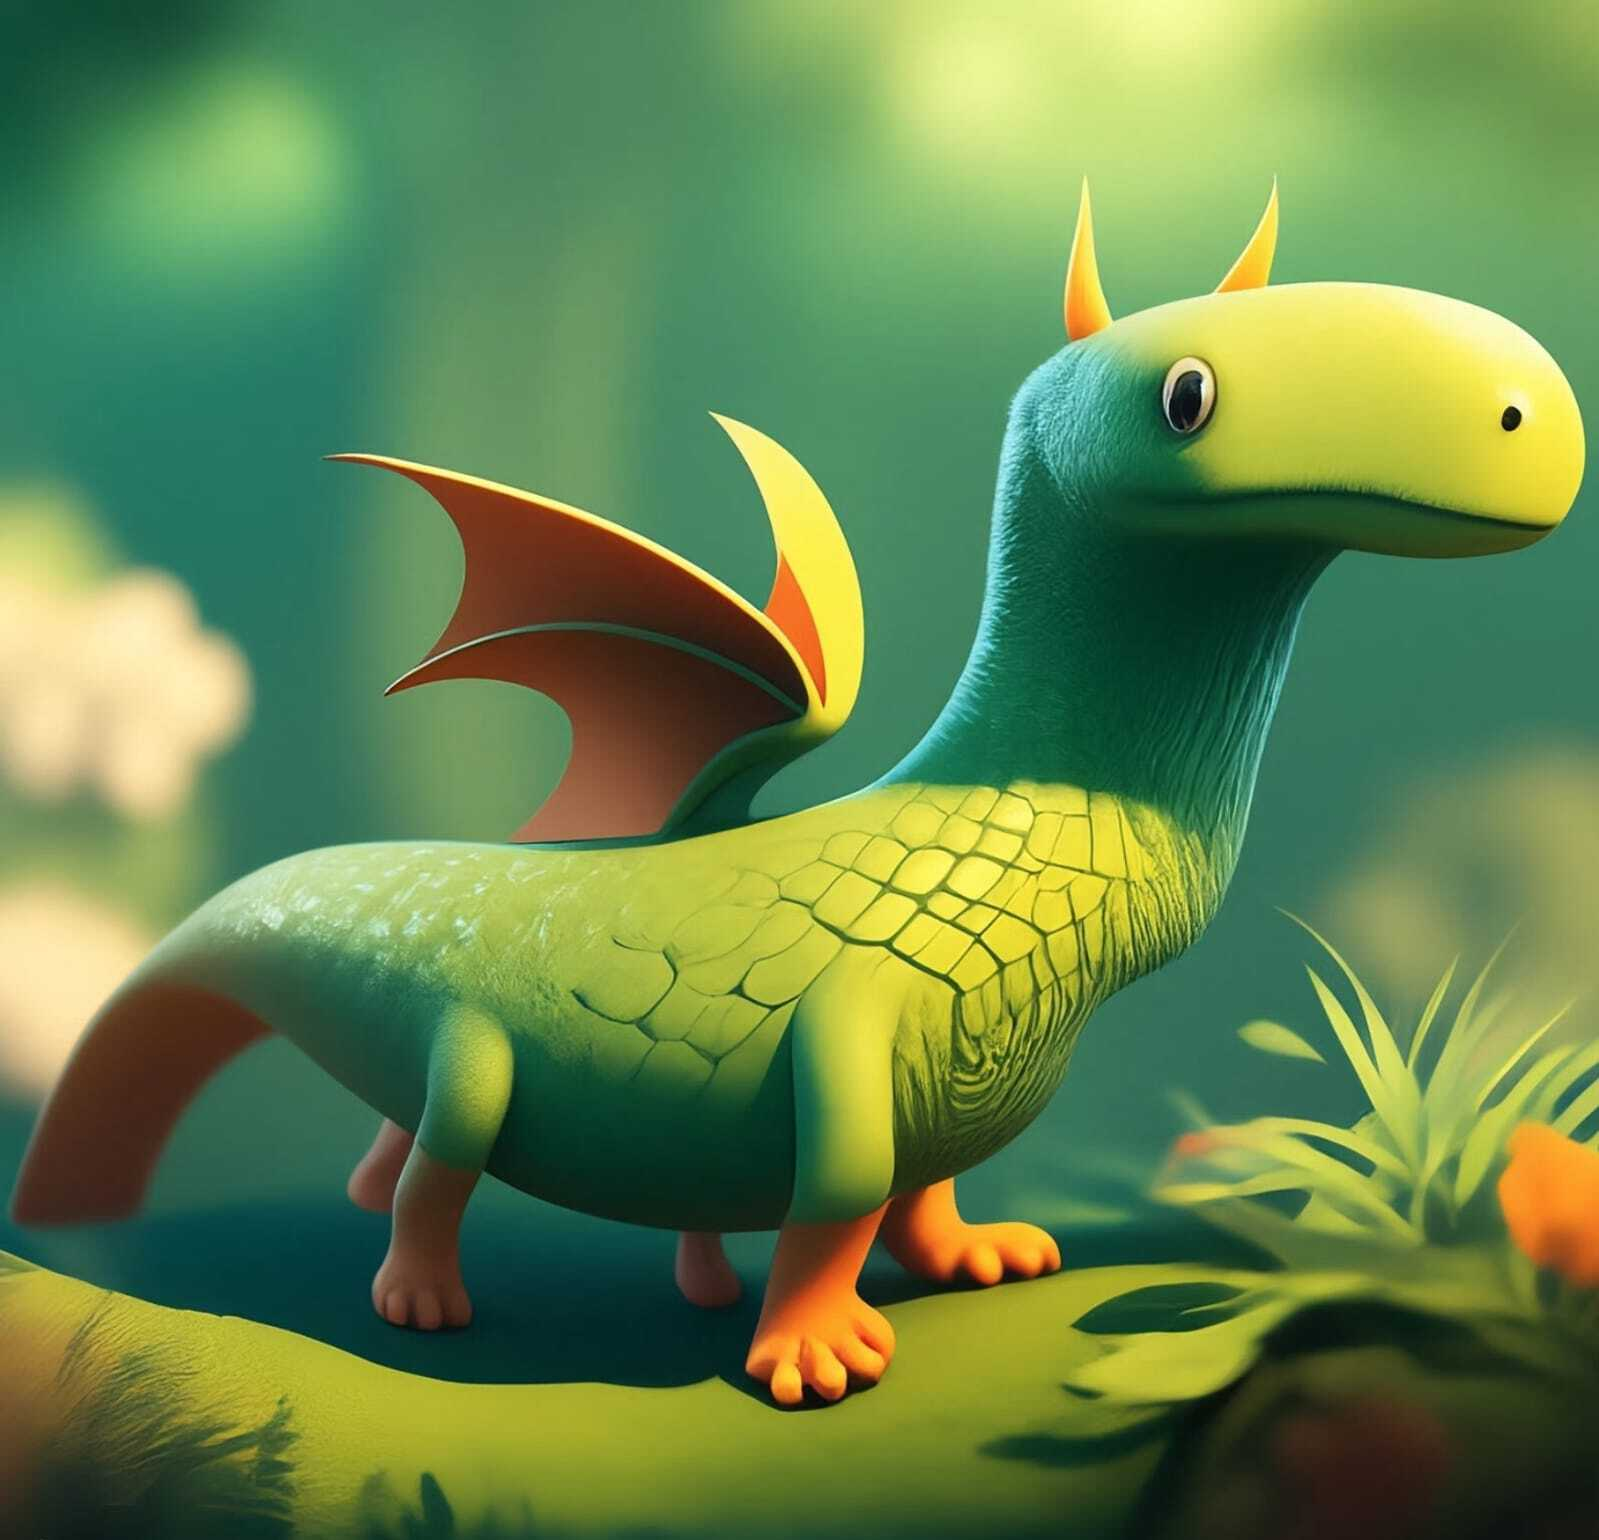
\includegraphics[width=6cm]{cover}
\end{center}
}

% theorem commands
\newtheoremstyle{c_remark}
	{}	% Space above
	{}	% Space below
	{}% Body font
	{}	% Indent amount
	{\bfseries}	% Theorem head font
	{}	% Punctuation after theorem head
	{.5em}	% Space after theorem head
	{\thmname{#1}\thmnumber{ #2}\thmnote{ \normalfont{\text{(#3)}}}}	% head content
\newtheoremstyle{c_definition}
	{3pt}	% Space above
	{3pt}	% Space below
	{}% Body font
	{}	% Indent amount
	{\bfseries}	% Theorem head font
	{}	% Punctuation after theorem head
	{.5em}	% Space after theorem head
	{\thmname{#1}\thmnumber{ #2}\thmnote{ \normalfont{\text{(#3)}}}}	% head content
\newtheoremstyle{c_plain}
	{3pt}	% Space above
	{3pt}	% Space below
	{\itshape}% Body font
	{}	% Indent amount
	{\bfseries}	% Theorem head font
	{}	% Punctuation after theorem head
	{.5em}	% Space after theorem head
	{\thmname{#1}\thmnumber{ #2}\thmnote{ \text{(#3)}}}	% head content

\ifcsname c@english\endcsname
	\theoremstyle{plain}
	\newtheorem{theorem}{Theorem}[section]
	\newtheorem{lemma}[theorem]{Lemma}
	\newtheorem{proposition}[theorem]{Proposition}
	\newtheorem*{proposition*}{Proposition}
	%\newtheorem{corollary}[theorem]{אין חלופה עברית}

	\theoremstyle{definition}
	\newtheorem{definition}[theorem]{Definition}
	\newtheorem*{definition*}{Definition}
	\newtheorem{example}{Example}[section]
	\newtheorem{exercise}{Exercise}[section]

	\theoremstyle{remark}
	\newtheorem*{remark}{Remark}
	\newtheorem*{solution}{Solution}
	\newtheorem{conclusion}[theorem]{Conclusion}
	\newtheorem{notation}[theorem]{Notation}
\else
	\theoremstyle{c_plain}
	\newtheorem{theorem}{משפט}[section]
	\newtheorem{lemma}[theorem]{למה}
	\newtheorem{proposition}[theorem]{טענה}
	\newtheorem*{proposition*}{טענה}
	%\newtheorem{corollary}[theorem]{אין חלופה עברית}

	\theoremstyle{c_definition}
	\newtheorem{definition}[theorem]{הגדרה}
	\newtheorem*{definition*}{הגדרה}
	\newtheorem{example}{דוגמה}[section]
	\newtheorem{exercise}{תרגיל}[section]

	\theoremstyle{c_remark}
	\newtheorem*{remark}{הערה}
	\newtheorem*{solution}{פתרון}
	\newtheorem{conclusion}[theorem]{מסקנה}
	\newtheorem{notation}[theorem]{סימון}
\fi

% Questions related commands
\newcounter{question}
\setcounter{question}{1}
\newcounter{sub_question}
\setcounter{sub_question}{1}

\ifcsname c@english\endcsname
	\newcommand{\question}[1][0]{
		\ifthenelse{#1 = 0}{}{\setcounter{question}{#1}}
		\section{Question \arabic{question}}
		\addtocounter{question}{1}
		\setcounter{sub_question}{1}
	}

	\newcommand{\subquestion}[1][0]{
		\ifthenelse{#1 = 0}{}{\setcounter{sub_question}{#1}}
		\subsection{Part \alph{sub_question}}
		\addtocounter{sub_question}{1}
	}
\else
	\newcommand{\question}[1][0]{
		\ifthenelse{#1 = 0}{}{\setcounter{question}{#1}}
		\section{שאלה \arabic{question}}
		\addtocounter{question}{1}
		\setcounter{sub_question}{1}
	}

	\newcommand{\subquestion}[1][0]{
		\ifthenelse{#1 = 0}{}{\setcounter{sub_question}{#1}}
		\subsection{סעיף \localecounter{letters.gershayim}{sub_question}}
		\addtocounter{sub_question}{1}
	}
\fi

% import lua and start of document
\directlua{common = require ('../common')}

\GetEnv{AUTHOR}

% headers
\author{\AUTHOR}
\date\today

\title{פתרון מטלה 05 --- מבנים אלגבריים (2), 80446}

\begin{document}
\maketitle
\maketitleprint[red]

\question{}
\subquestion{}
נוכיח שחבורה אבלית סופית היא מכפלה ישרה של חבורות ה־$p$־סילו שלה. \\
נסיק שאם $n = p_1^{k_1} \cdots p_r^{k_r}$ פירוק לחזקות ראשוניים שונים אז $\ZZ_{/ p_1^{k_1}} \times \cdots \times \ZZ_{/ p_r^{k_r}} \simeq \ZZ_{/n}$,
ואף שהאיזומורפיזם $\varphi$ המעיד על כך מקיים,
\[
	\varphi(\{ (x_1, \ldots, x_r) \mid \forall 1 \le i \le r, \langle x_i \rangle = \ZZ_{/ p_i^{k_i}} \})
	= \{ x \in \ZZ_{/n} \mid \langle x \rangle = \ZZ_{/n} \}
\]
\begin{proof}
	נניח ש־$p_1, \ldots, p_n$ הראשוניים המחלקים את $|G|$, עבור חבורה אבלית סופית $G$.
	נניח גם ש־$n_i$ מספר חבורות $p_i$־סילו של $G$.
	אנו יודעים שכל חבורות $p_i$־סילו הן צמודות אחת לשנייה ולכן אם $P, Q \le G$ חבורות $p_i$ סילו שלה אז קיים $g \in G$ כך ש־$g P g^{-1} = Q$.
	אבל $G$ אבלית ולכן לכל $h \in P$ נקבל $g p g^{-1} = p$ ונסיק ש־$P = Q$, כלומר $n_{p_i} = 1$.
	נגדיר $P_i \le G$ החבורה היחידה $p_i$־סילו של $G$ לכל $i$.

	נראה שאכן $G \simeq P_1 \times \cdots \times P_n$.
	אנו כבר יודעים שמתקיים $G = P_1 \cdots P_n$ מאבליות. \\
	נניח ש־$i < j \le n$ ונבחן את $P_i \cap P_j$.
	אם קיים $e \ne g \in P_i \cap P_j$ נקבל שהסדר של $g$ הוא $p_i$ וגם $p_j$ ולכן $p_i = p_j$ בסתירה להגדרתם, ולכן $P_i \cap P_j = \{ e \}$ לכל $i \ne j$. \\
	עוד נבחין כי ממשפט סילו השני $P_i \trianglelefteq G$ לכל $i \le n$. \\
	נסיק מהאפיון למכפלות ישרות ש־$G \simeq P_1 \times \cdots \times P_n$.

	מאפיון של חבורות $\ZZ_{/n}$ אנו יודעים ש־$H \le \ZZ_{/n}$ אם ורק אם $H \simeq \ZZ_{/d}$ עבור $d \mid n$, ולכן נסיק ש־$P_i = \ZZ_{p_i^{k_1}}$ לכל $i$ וכאשר $k_i$ מקסימלי בחלוקה $p_i^{k_i} \mid n$.
	נניח ש־$\varphi : \ZZ_{/ p_1^{k_1}} \times \cdots \times \ZZ_{/ p_r^{k_r}} \to \ZZ_{/n}$ האיזומורפיזם המעיד על כך.
	נניח ש־$(x_1, \ldots, x_r)$ איברים כך ש־$\langle x_i \rangle = \ZZ_{p_i^{k_i}}$ לכל $i \le r$.
	אז הסדר של $(x_1, \ldots, x_r)$ הוא $n$ ולכן נוכל להסיק שגם $\varphi(x_1, \ldots, x_r)$ מסדר $n$, כלומר בהכרח $\langle \varphi(x_1, \ldots, x_r) \rangle = \ZZ_{/n}$ בלבד. \\
	מהצד השני נניח ש־$x \in \ZZ_{/n}$ כך ש־$\langle x \rangle = \ZZ_{/n}$.
	נגדיר גם $x_i = \pi_i(x)$ עבור הומומורפיזם ההטלה $\pi_i : \ZZ_{/n} \to \ZZ_{/p_i^{k_i}}$ לכל $i$.
	משיקולי סדר דומים בהכרח $\langle x_i \rangle = \ZZ_{/p_i^{k_1}}$ ולכן נקבל שאכן מתקיים,
	\[
		\varphi(\{ (x_1, \ldots, x_r) \mid \forall 1 \le i \le r, \langle x_i \rangle = \ZZ_{/ p_i^{k_i}} \})
		= \{ x \in \ZZ_{/n} \mid \langle x \rangle = \ZZ_{/n} \}
	\]
	כפי שרצינו להוכיח.
\end{proof}

\subquestion{}
נראה ש־$\aut(\ZZ / n \ZZ) \simeq {(\ZZ / n \ZZ)}^\times$,
וכן שאם $n = p_1^{k_1} \cdots p_r^{k_r}$ פירוק לחזקות ראשוניים שונים אז,
\[
	{(\ZZ / n \ZZ)}^\times
	\simeq {(\ZZ / p_1^{k_1} \ZZ)}^\times \times \cdots \times {(\ZZ / p_r^{k_r} \ZZ)}^\times
\]
\begin{proof}
	נגדיר את ההעתקה $\sigma : \aut(\ZZ / n \ZZ) \to {(\ZZ / n \ZZ)}^\times$, על־ידי $\sigma(\varphi) = \varphi(1)$.
	נבחין כי לכל $\varphi, \psi \in \aut(\ZZ / n \ZZ)$,
	\[
		\sigma(\varphi \circ \psi)
		= \varphi(\psi(1))
		= \varphi(\underline{k})
		= k \cdot \varphi(1)
		= \varphi(1) \cdot \psi(1)
	\]
	כאשר $\underline{k}$ הנמרטור המייצג את $\psi(1)$.
	נסיק ש־$\sigma$ הומומורפיזם חבורות, נרצה להראות שהוא חד־חד ערכי ועל. \\
	נניח ש־$\sigma(\varphi) = \sigma(\psi)$, אז $\varphi(1) = \psi(1)$ ונסיק ישירות ש־$\varphi = \psi$, לכן $\sigma$ חד־חד ערכית. \\
	יהי $k \in {(\ZZ / n \ZZ)}^\times$, אז נגדיר $\varphi(x) = k \cdot x$, זהו אוטומורפיזם פנימי וכן $\sigma(\varphi) = k$, ולכן $\sigma$ על. \\
	נסיק ש־$\aut(\ZZ / n \ZZ) \simeq {(\ZZ / n \ZZ)}^\times$.

	אנו יודעים שאם $G = H \times K$ אז $\aut G \simeq \aut H \times \aut K$ ישירות מהגדרת אוטומורפיזם והרכבת איזומורפיזם עליו.
	נוכל להרחיב את המכפלה הזו לכל כמות סופית של מכפלות, ונסיק,
	\[
		{(\ZZ / n \ZZ)}^\times
		\simeq \aut(\ZZ / n \ZZ)
		\simeq \aut(\ZZ / p_1^{k_1} \ZZ) \times \cdots \times \aut(\ZZ / p_r^{k_r} \ZZ)
		\simeq {(\ZZ / p_1^{k_1} \ZZ)}^\times \times \cdots \times {(\ZZ / p_r^{k_r} \ZZ)}^\times
	\]
	ואכן קיים איזומורפיזם.
\end{proof}

\subquestion{}
תהי $(A, +)$ חבורה אבלית סופית.
נסיק שאם לכל $p$ ראשוני כך ש־$p \mid |A|$ מתקיים,
\[
	A[p]
	= \{ a \in A \mid \exists k \in \NN, p^k a = 0 \}
\]
היא ציקלית, אז $A$ ציקלית.
\begin{proof}
	נתון כי $A[p]$ ציקלית לכל $p$, ונבחין כי $p^k = 0$ עבור $k$ מקסימלי כלשהו, לכן $1 \in A[0]$, ונסיק ש־$|A[p]| = p^k$, כלומר זוהי חבורת $p$־סילו של $A$.
	אילו נבחר $(1, \ldots, 1)$ אז $\varphi(1, \ldots, 1) = x \in A$ עבור $\varphi$ מסעיף א'.
	אבל מהמסקנה של אותו סעיף נובע ש־$\langle x \rangle = A$, כלומר $x$ מעיד על הציקליות של $A$.
\end{proof}

\subquestion{}
נראה שאם $(A, +)$ חבורה אבלית מסדר $p^n$ עבור $p$ ראשוני כלשהו, וגם של־$A$ יש תת־חבורה ציקלית יחידה מסדר $p$, אז $A$ ציקלית.
\begin{proof}
	יהי $a \in A$, ונניח כי $a \notin \langle b \rangle$ עבור $b \in A$ כך ש־$o(b) = p$.
	אז $o(a) \ne p$, אחרת נקבל ש־$\langle a \rangle$ מסדר $p$ ולכן $a \in \langle b \rangle$.
	אילו $o(a) = p^k$ עבור $1 < k < n$ אז נקבל $\langle a \rangle$ חבורה ציקלית מסדר $p^k$.
	אבל מאפיון חבורות־$p$ אנו יודעים שקיימת $H \le \langle a \rangle \le A$ כך ש־$|H| = p$, ולכן $H$ ציקלית, אבל $a \notin \langle b \rangle$ ולכן $H \ne \langle b \rangle$ וקיבלנו סתירה להנחה.
	לכן בהכרח $k = n$ ונובע ש־$A$ עצמה ציקלית.
\end{proof}

\subquestion{}
נראה שאם $(A, +)$ חבורה אבלית כך שלכל $p \mid A$ מתקיים ש־$A[p]$ אבלית, עם תת־חבורה ציקלית יחידה מסדר $p$, אז $A$ ציקלית.
\begin{proof}
	מסעיף ד' נובע ש־$A[p]$ ציקלית לכל $p \mid |A|$, ומסעיף ג' נובע ש־$A$ ציקלית.
\end{proof}

\question{}
נניח ש־$p_1, \ldots, p_n$ ראשוניים זרים, נוכיח בסעיפים הבאים כי,
\[
	\QQ(\sqrt{p_1} + \cdots + \sqrt{p_n})
	= \QQ(\sqrt{p_1}, \ldots, \sqrt{p_n}) = L
\]
\subquestion{}
נראה שאם $\epsilon_1, \ldots, \epsilon_n \in \{ \pm 1 \}$ אז יש אוטומורפיזם, $\varphi_n$, של $L$ ששולח את $\sqrt{p_i}$ ל־$\epsilon_i \sqrt{p_i}$ לכל $i$.
\begin{proof}
	נראה את הטענה באינדוקציה על $n$.
	עבור $n = 0$ הטענה טריוויאלית.

	נניח שקיים אוטומורפיזם של $L_n = \QQ(\sqrt{p_1}, \ldots, \sqrt{p_n})$ השולח את $\sqrt{p_i}$ ל־$\epsilon_i \sqrt{p_i}$ ונראה שעבור $p_{n + 1}$ ו־$\epsilon_{n + 1}$ ניתן להרחיב את האוטומורפיזם הזה על,
	\[
		L_{n + 1} = L_n(\sqrt{p_{n + 1}})
		\simeq L_n[x] / (x^2 - p_{n + 1})
	\]
	כאשר האיזומורפיזם האחרון נובע מהעובדה שזהו הפולינום המינימלי של $\sqrt{p_{n + 1}}$.
	נסיק אם כך ש־$L_n(\sqrt{- p_{n + 1}}) \simeq L_n[x] / (x^2 - p_{n + 1})$ ולכן נובע ש־$L_{n + 1} \simeq L_n(\epsilon_i \sqrt{p_{n + 1}})$.
	משאלה 3 במטלה 3 נוכל להסיק אף ש־$L_{n + 1} = L_n(\epsilon_i \sqrt{p_{n + 1}})$.

	נגדיר $\varphi_{n + 1} : L_{n + 1} \to L_{n + 1}$ על־ידי $\varphi_{n + 1} \restriction L_n = \varphi_n$ וכן $\varphi_{n + 1}(\sqrt{p_{n + 1}}) = \epsilon_i \sqrt{p_{n + 1}}$.
	זהו $L_n$־הומומורפיזם.
	מהעובדה שיש שוויון בין השדות, נוכל להסיק שבפרט קיים אוטומורפיזם, וזהו אוטומורפיזם כזה.
\end{proof}

\subquestion{}
נראה שאם $\epsilon_1, \ldots, \epsilon_n \in \{ \pm 1 \}$ אז $\sum_{i = 1}^n \epsilon_i \sqrt{p_i}$ צמוד של $\sum_{i = 1}^n \sqrt{p_i}$ מעל $\QQ$,
ונסיק שיש להם את אותו הפולינום המינימלי.
\begin{proof}
	אנו יודעים כי קיים אוטומורפיזם $\varphi : L \to L$ כך ש־$\varphi(\sqrt{p_i}) = \epsilon_i \sqrt{p_i}$ לכל $i$.
	\[
		\varphi\left(\sum_{i = 1}^n \sqrt{p_i}\right)
		= \sum_{i = 1}^n \epsilon_i \sqrt{p_i}
	\]
	מהגדרת $\varphi$.
	אבל מלמה מההרצאה נובע בהכרח שבשדות נורמליים איברים עוברים לצמודים שלהם בלבד.
	אנו טוענים ש־$L$ נורמלית, זאת שכן נוכל לאפיין באותו אופן של סעיף א' את כל האוטומורפיזמים של $L$ מעל $\overline{L}$, ונקבל שהתמונה תמיד זהה.
	נסיק אם כך שאכן שני האיברים צמודים, ולכן מהגדרת צמידות יש להם פולינום מינימלי משותף.
\end{proof}

\subquestion{}
נחשב את דרגת הפולינום המינימלי, $f$, של $\sqrt{p_1} + \cdots + \sqrt{p_n}$ ונסיק את הטענה הראשית.
\begin{proof}
	נבחין כי לכל בחירת $\epsilon_i$ נקבל ש־$\epsilon_1 \sqrt{p_1} + \cdots + \epsilon_n \sqrt{p_n}$ איבר צמוד של $\sqrt{p_1} + \cdots + \sqrt{p_n}$.
	נובע אם כך ש־$\deg_\QQ f \ge 2^n$.
	אבל מתכונות של פולינום מינימלי שראינו בהרצאה ידוע גם כי $\deg_\QQ f \le 2^n$, על־ידי שימוש בתכונות על חסמי פולינום מינימלי ביחס לפעולות החיבור והכפל, ולכן $\deg_\QQ f = 2^n$.

	אנו יודעים שדרגת $L$ היא $2^n$ כמגדל הרחבות, וכן $\sqrt{p_1} + \cdots + \sqrt{p_n} \in L$, ולכן נוכל להסיק שמתקיים,
	\[
		\QQ(\sqrt{p_1} + \cdots + \sqrt{p_n})
		= \QQ(\sqrt{p_1}, \ldots, \sqrt{p_n}) = L
	\]
	כפי שרצינו.
\end{proof}

\question{}
בכל סעיף נגדיר $f \in \QQ[x]$ ונוכיח ש־$f$ אי־פריק.
נניח ש־$\alpha \in \CC$ שורש של $f$ ונגדיר $K = \QQ(\alpha)$, נבדוק האם $K / A$ הרחבה נורמלית.

\subquestion{}
נגדיר $f(x) = x^4 + x^3 + x^2 + x + 1 = \frac{x^5 - 1}{x - 1}$.
\begin{solution}
	$f$ הוא הפולינום הציקלוטומי מסדר $5$, זהו סדר ראשוני ולכן מטענה מהרצאה נובע שהוא אי־פריק. \\
	השורשים של $f$ מעל $\CC$ הם $\omega^n$ עבור $\omega = \exp(\frac{2\pi i n}{5})$ ו־$1 \le n \le 4$.
	לכל $q \in \QQ$ אנו יודעים כי $f_{q / \QQ}$ מתפצל לחלוטין מעל $\QQ(\alpha)$ ולכן עלינו לבדוק רק את $\omega$.
	אנו יודעים כי $f_{\omega / \QQ}(x) = x^5 - 1$, מעקרון שובך היונים והעובדה ש־$o(\alpha) = 5$ נסיק ש־$\omega \in \QQ(\omega^n)$ ולכן $f_{\omega / \QQ}$ מתפצל לחלוטין בשדה זה, ונסיק שהוא נורמלי.
\end{solution}

\subquestion{}
נגדיר $f(x) = x^4 - 7x^2 + 7$.
\begin{solution}
	נבחין כי,
	\[
		x^2
		= \frac{7 \pm \sqrt{49 - 28}}{2}
		= \frac{7 \pm \sqrt{21}}{2}
	\]
	ולכן,
	\[
		x = \pm \sqrt{\frac{7 \pm \sqrt{21}}{2}}
	\]
	מבדיקה ישירה נקבל שאף מכפלת שורשים של $f$ היא לא רציונלית, ולכן נוכל להסיק ש־$f$ אי־פריק מעל $\QQ$.

	יהי $\alpha$ שורש של $f$.
	נסמן $\beta = \alpha^2$, נסמן,
	\[
		\beta_1 = \frac{7 + \sqrt{21}}{2},
		\quad
		\beta_2 = \frac{7 - \sqrt{21}}{2}
	\]
	ונניח בלי הגבלת הכלליות ש־$\alpha = \beta_1$ (אחרת ההוכחה זהה).
	נבדוק אם $\sqrt{\beta_2} \in \QQ(\alpha) = \QQ(\sqrt{\beta_1})$.
	\[
		\sqrt{\beta_2}
		= \sqrt{7 - \beta_1}
	\]
	ולכן נוכל להסיק $f_{\sqrt{\beta_2} / \QQ(\alpha)} = x^2 - 7 + \sqrt{\alpha}$ וזהו פולינום אי־פריק ולכן לא כל שורשי $f$ ב־$\QQ(\alpha)$ ונובע שהוא לא נורמלי מעל $\QQ$.
\end{solution}

\subquestion{}
נגדיר $f(x) = x^4 - x - 1$.
\begin{solution}
	אילו $f$ פריק ב־$\QQ$ אז הוא פריק גם ב־$\FF_2[x]$ (1.4.2).
	נבחין כי ב־$\FF_2[x]$ גם $f(x) = x^4 + x + 1$.
	בהצבה נקבל $f(x) = 1$ לכל $x \in \FF_2$, ולכן אם $f$ פריק אז הוא מכפלת פולינומים מסדר 2.
	אבל הוא לא מכפלה של $x^2, x^2 + x, x^2 + 1$ שכן להם יש שורש, ונשאר לבדוק את $x^2 + x + 1$.
	אבל ישירות מחלוקת פולינומים נקבל שפולינום זה לא מחלק את $f$ ולכן $f$ אי־פריק מעל $\FF_2[x]$ ומהמשפט לא פריק ב־$\QQ$.

	נבחין כי $f'(x) = 4x^3 - 1$ ולכן הנגזרת מונוטונית עולה ונסיק של־$f$ יש אפס או שני שורשים בלבד, אבל בהצבה נקבל $f(0) = -1 < 0$ וכן $f(2) = 13 > 0$ ולכן יש בדיוק שני שורשים ל־$f$.
	שורשים אלה הם שניהם ממשיים, אבל משימוש במשפט רושה על תחום פתוח שלא כולל את הציר הממשי והפולינום $g(z) = z^4$ נוכל להסיק שיש לפחות שורש מרוכב אחד, ובהתאם למסקנה מהתרגול ההרחבה $\QQ(\alpha) / \QQ$ לא נורמלית.
\end{solution}

\question{}
יהי $K$ שדה כך ש־$\mu_\infty$ מתפצלת, ולכן לכל שורש יחידה $z \in \overline{K}$ גם $z \in K$.
נסמן $p = \operatorname{char}(K)$ אם המציין של $K$ חיובי ו־$p = 1$ אחרת. \\
נוכיח כי $\mu_\infty(K) \simeq \QQ / (\ZZ[\frac{1}{p}])$.
\begin{proof}
	במקרה $p = 1$ אנו רוצים להראות כי $\mu_\infty(K) \simeq \QQ / \ZZ$.
	לכל $n \in \NN$, כל $\mu_n \le \mu_\infty$ היא חבורה ציקלית, נקבע את אחד מהשורשים הפרימיטיביים ב־$\mu_n$, נסמן $\omega_n$,
	ונגדיר את $\varphi_n : \mu_n \to \QQ / \ZZ$ על־ידי $\varphi_n(\zeta) = \frac{k}{n}$ כאשר $\zeta = \omega_n^k$.
	עתה נגדיר $\varphi : \mu_\infty(K) \to \QQ / \ZZ$, לכל $\zeta \in \mu_\infty$ נבחר $n$ כך ש־$\zeta \in \mu_n$ ונגדיר $\varphi(\zeta) = \varphi_n(\zeta)$.
	אנו יודעים כבר כמסקנה מהרצאה ש־$\varphi$ כזו היא מוגדרת היטב, נשאר להראות שהיא איזומורפיזם.
	לכל $\zeta, \eta \in \mu_\infty$ קיים $n \in \NN$ כך ש־$\zeta, \eta \in \mu_n$, זאת על־ידי בחירת $\operatorname{lcm}(m, l)$ עבור סדרים של שני האיברים.
	אז מתקיים,
	\[
		\varphi(\zeta \cdot \eta)
		= \varphi_n(\zeta \cdot \eta)
		= \frac{k_1 + k_2}{n}
		= \frac{k_1}{n} + \frac{k_2}{n}
		= \varphi_n(\zeta) + \varphi_n(\eta)
		= \varphi(\zeta) + \varphi(\eta)
	\]
	ונסיק ש־$\varphi$ הומומורפיזם. \\
	נניח ש־$\zeta, \eta \in \mu_\infty$ כך ש־$\zeta \ne \eta$, אז,
	\[
		\varphi(\zeta)
		= \frac{k_1}{n}
		\ne \frac{k_2}{n}
		= \varphi(\eta)
	\]
	ולכן נסיק חד־חד ערכיות. \\
	לכל $\frac{k}{n}$ אנו יודעים ש־$1 \in K$ שורש יחידה מסדר $n$ וכן שהוא מתפצל לחלוטין, ולכן נבחר $\zeta \in \mu_n$ מתאימה ונקבל $\varphi(\zeta) = \frac{k}{n}$ ונסיק על, לכן,
	\[
		\mu_\infty(K)
		\simeq \QQ / \ZZ
	\]

	במקרה $p > 1$ ההוכחה דומה ומשתמשת בלמה 6.1.7.
	אנו יודעים ש־$\mu_n \simeq \ZZ / m \ZZ$ עבור $n = p^l m$ כך ש־$\gcd(m, p) = 1$.
	בהתאם גם $m = \frac{n}{p^l}$ ונוכל ליצור העתקה $\varphi_n : \mu_n \to \QQ /(\ZZ[\frac{1}{p}])$.
	שאר ההוכחה זהה.
\end{proof}

\end{document}
